    \begin{minipage}{0.45\textwidth}
        \centering
        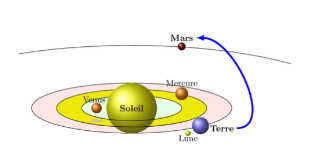
\includegraphics[width=\textwidth]{../../assets/images/figure-2.png}
          \end{minipage}
    \hfill
    % Hình thứ hai
    \begin{minipage}{0.45\textwidth}
        \centering
        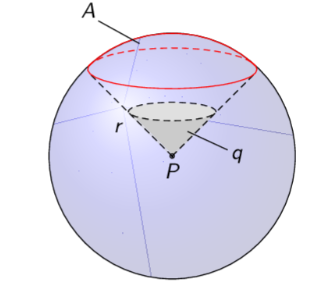
\includegraphics[width=0.7\textwidth]{../../assets/images/figure-3.png}
    \end{minipage}
    \caption{Hình đôi}
        \label{fig:image3}
\end{figure}

\subsection{Tiểu mục 2}

% nội dung này có thể tham khảo giáo trình ĐSTT và HH2
\section{Mục 2}
\subsection{Tiểu mục 1}

\subsection{Tiểu mục 2}

\noindent % Để loại bỏ thụt lề đầu dòng
\begin{minipage}{0.4\textwidth} % Phần hình ảnh (40% chiều rộng trang)
    \centering
    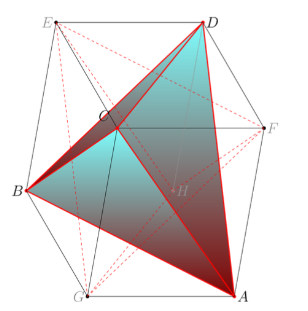
\includegraphics[width=\textwidth]{../../assets/images/figure-1.png} % Đường dẫn tới ảnh
    \captionof{figure}{Hình minh họa} % Chú thích cho hình
    \label{fig:image}
\end{minipage}%
\hfill % Thêm khoảng cách giữa hình và chữ
\begin{minipage}{0.55\textwidth} % Phần văn bản (55% chiều rộng trang)
    Đây là đoạn văn bản mô tả hình ảnh. Bạn có thể viết bất kỳ nội dung nào ở đây để giải thích hoặc chú thích cho hình bên cạnh. Sử dụng phần trăm chiều rộng hợp lý để tối ưu bố cục tài liệu.
\end{minipage}
\chapter*{KẾT LUẬN}
\addcontentsline{toc}{chapter}{KẾT LUẬN}

% Nội dung kết luận của luận văn sẽ được viết ở đây
% Tóm tắt những kết quả đạt được, ý nghĩa và hướng phát triển
\begin{thebibliography}{70}
\section*{\hskip-\leftmargin Tiếng Việt}
\bibitem{1} Nguyễn Văn A (1999). \textit{Tên sách in nghiêng}, Tên NXB.
\bibitem{2} Nguyễn Văn B và Trần Thị C (1982). Tên bài báo, \textit{Tên tạp chí in nghiêng}, Số xuất bản, Trang 11--20.
\bibitem{3} Nguyễn Văn C (2022). \textit{Tên luận văn in nghiêng}, Luận văn Thạc sĩ hay Đại học, Tên Trường Đại học.

\section*{\hskip-\leftmargin Tiếng Anh}
\bibitem{4} D. Alibaba (1982). \textit{The tittle of book}, Publishing House.
\bibitem{5} F. Colony (2006). The tittle of paper, \textit{Journal's name}, Vol. xx, page 11--20.
\bibitem{} E. Marcos (2024). \textit{Thesis's tittle}, Master's thesis or Bachelor's thesis, Bonba University.
%\bibitem{8} 
\end{thebibliography}
%HƯỚNG DẪN CÁCH GHI TLTK XÓA BỎ KHI HOÀN THANH LUẬN VĂN
\begin{table*}
\centering
\begin{tabular}{|l|l|l|}
    \hline
      Loại trích dẫn   & Trích dẫn trong ngoặc đơn (Parenthetical citation) & Trích dẫn trong câu 
(Narrative citation)
\\
     \hline
       \textbf{Một tác giả}
       
Ghi tác giả và năm
  & (Hường, 2013)
  
(Tain, 1999)
 & Hường (2013)
 
Tain (1999)
\\
    \hline
   \textbf{Hai tác giả}
   
Ghi hai tác giả và năm		
      & (Deharveng $\&$ Bedos, 2000) 
      
(Hồ $\&$ Lư, 2003) & Deharveng and Bedos (2000)

Hồ và Lư (2003)\\
         \hline
       \textbf{Ba tác giả trở lên}
       
Ghi tác giả đầu tiên, theo sau là ``và ctv.'' hoặc ``et al.'' và năm 
  & (Aron et al., 2019)
  
(Hiền và ctv., 2016)

*``và ctv.'', ``et al.'' không viết in nghiêng
 & Aron et al. (2019)
 
Hiền và ctv. (2016)
\\
\hline
  \textbf{Tác giả là một cơ quan, tổ chức}
  
Ghi tên cơ quan và năm (Tên cơ quan có thể viết tắt nếu được trích dẫn hơn một lần trong bài)
       &  (United States Government Accountability Office, 2019)

*Trích dẫn lần đầu:
 (Food and Agriculture Organization of the United Nations [FAO], 1977)
 
